\documentclass{beamer}
\usepackage{config}

%Information to be included in the title page:
\title[Git collaboratif]{Git à plusieurs : mode d'emploi}
\author{Florian Legendre}
\institute{Université de Poitiers}
\date{Année 2020 - 2021}
\logo{
\includegraphics[scale=0.1]{UP.png}}


%%% ============================================================= %%%
%%% ====================== Début des diapos ===================== %%%
%%% ============================================================= %%%

\begin{document}

\frame{\titlepage}

\begin{frame}
\frametitle{Table of Contents}
\tableofcontents[hideallsubsections]
\end{frame}




%% --------------------- %%
%%        SECTION        %%
%% --------------------- %%
\AtBeginSection[]
{
  \begin{frame}
    \frametitle{Table of Contents}
    \tableofcontents[sectionstyle=show/hide,subsectionstyle=show/show/hide]
  \end{frame}
}

\section{Rappels sur les conflits d'édition}

% Subsection:
\subsection{Quelques remarques préliminaires}
\begin{frame}{Git n'est pas GitHub!}

À l'instar des branches où je considérais que vous aviez un dépôt distant et où je vous  montrais comment configurer vos branches locales/distantes depuis Git, ici je vais vous présenter une dernière notion de Git qui est indépendante du choix de dépôt distant que vous ferez.\\
\medskip

Cette notion est celle de conflit d'éditions. Bien que le mot "conflit" puisse faire peur il s'agit de quelque-chose de tout à fait ordinaire quand on travaille à plusieurs sur un même projet. Git simplifie grandement la gestion de ces conflits.\\

\end{frame}

% Subsection:
\subsection{Rappel de la notion de conflits d'édition}
\begin{frame}{Rappel du problème}
\begin{center}
    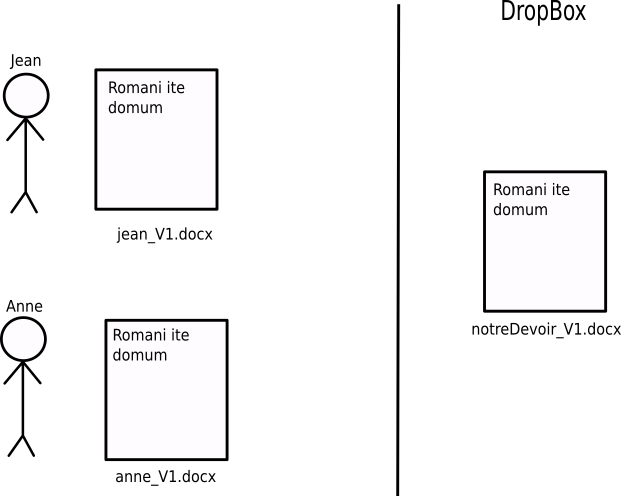
\includegraphics[scale=0.4]{lastScenario/lastScenario_init.png}
\end{center}
\end{frame}

\begin{frame}{Rappel du problème}
\begin{center}
    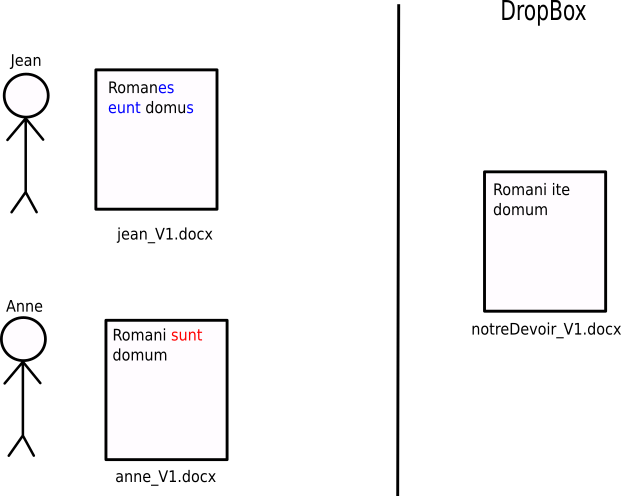
\includegraphics[scale=0.4]{lastScenario/lastScenario_conflict1.png}
\end{center}
\end{frame}

\begin{frame}{Rappel du problème}
\begin{center}
    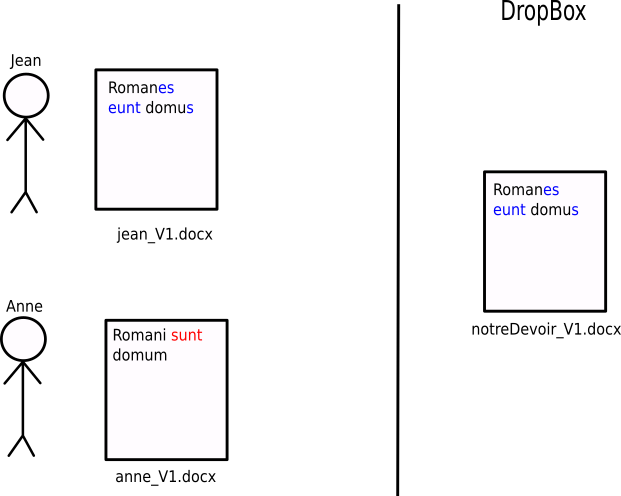
\includegraphics[scale=0.4]{lastScenario/lastScenario_conflict2.png}
\end{center}
\end{frame}

\begin{frame}{Rappel du problème}
\begin{center}
    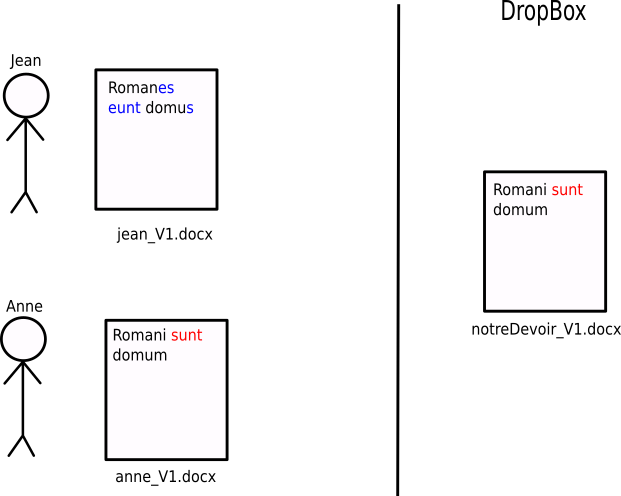
\includegraphics[scale=0.4]{lastScenario/lastScenario_conflict3.png}
\end{center}
\end{frame}

\begin{frame}{Rappel de la solution "à la main"}
\begin{center}
    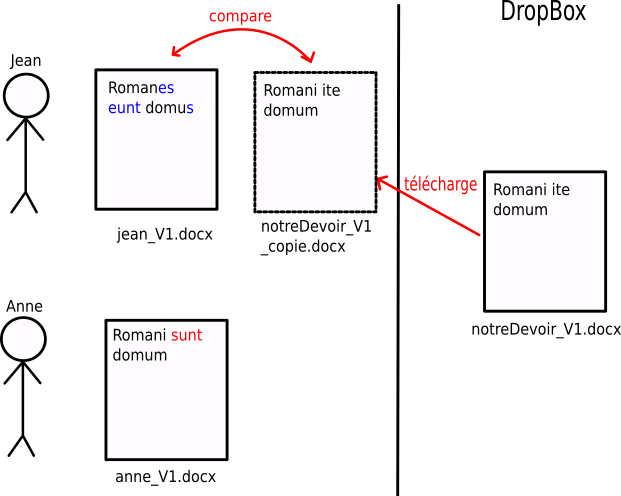
\includegraphics[scale=0.4]{lastScenario/lastScenario_pullpush1.png}
\end{center}
\end{frame}

\begin{frame}{Rappel de la solution "à la main"}
\begin{center}
    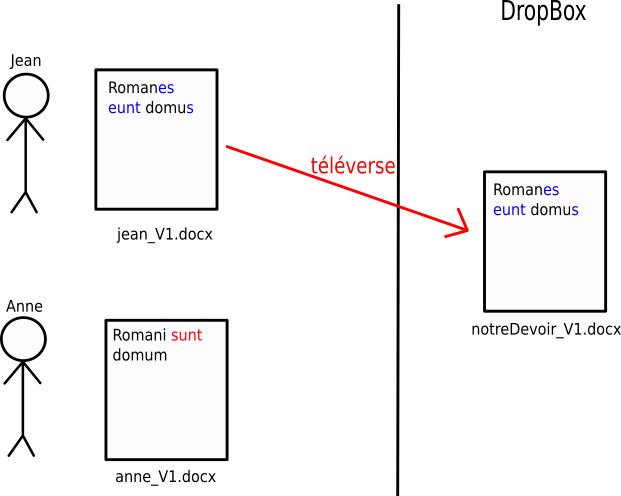
\includegraphics[scale=0.4]{lastScenario/lastScenario_pullpush2.png}
\end{center}
\end{frame}

\begin{frame}{Rappel de la solution "à la main"}
\begin{center}
    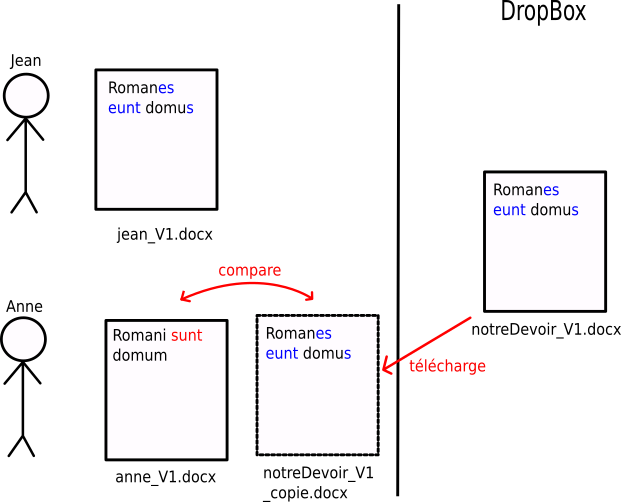
\includegraphics[scale=0.4]{lastScenario/lastScenario_pullpush3.png}
\end{center}
\end{frame}


% Subsection:
\subsection{Quel est le rôle de Git dans la gestion de ces conflits?}
\begin{frame}{Rôle de Git}

Git ne peut pas décider à votre place de ce qui doit être supprimé ou gardé! Ou alors nous perdons tous notre travail car les ordinateurs peuvent coder...\\
\medskip

Mais Git peut vous indiquer dans quels fichiers et à quelles lignes vos deux versions sont en conflit. 
    
\end{frame}


%% --------------------- %%
%%        SECTION        %%
%% --------------------- %%
\AtBeginSection[]
{
  \begin{frame}
    \frametitle{Table of Contents}
    \tableofcontents[sectionstyle=show/hide,subsectionstyle=show/show/hide]
  \end{frame}
}

\section{Gestion des conflits d'édition avec Git}


% Subsection:
\subsection{Présentation d'un conflit détecté par Git}
\begin{frame}[fragile]{Un conflit sur Git}
Un exemple illustrant la détection automatique de conflits d'édition entre plusieurs collaborateurs:
\begin{mdframed}[style=Bash]
\begin{lstlisting}[style=Bash, caption={Exemple de détection automatique de conflit d'édition}]
<<<<<<< HEAD
VisuRepereMokka(markers.Potence,Rpotence_R0,c3d,'Rpotence_R0')
=======
VisuRepereMokla(markers.Potence,Rpotence_R0,c3d,'Rpotence_R0')
>>>>>>> travail_de_monOuma_collegue
\end{lstlisting}
\end{mdframed}
\end{frame}


% Subsection:
\subsection{Résolution d'un conflit d'édition}
\begin{frame}{Résolution d'un conflit d'édition}
    
\end{frame}


\end{document}